\documentclass[letterpaper, 11pt]{article}

\usepackage{lastpage, url, marginnote, siunitx, circuitikz, kantlipsum}

\usepackage{geometry}
\geometry{hscale=.6, vscale=.8, hmarginratio=2:1, vmarginratio=1:1, marginparwidth=.18\paperwidth, ignoremp}
%\geometry{marginparwidth=.1\paperwidth}

%\usepackage[T1]{fontenc}

\usepackage[explicit]{titlesec}
\titlespacing*{\section}{\dimexpr -\marginparsep-\marginparwidth}{*4}{*1}
\titleformat{\section}[runin]{\large\bfseries\titlerule[.5pt]\filright}{\makebox[1em][c]{\thesection}}{1em}{\parbox[t]{\dimexpr\marginparwidth-2em}{#1}\hskip\marginparsep\mbox{}}[\newline]

%\titlespacing*{\subsection}{\dimexpr -\marginparsep-\marginparwidth}{*4}{*1}
%\titleformat{\subsection}[runin]{\large\bfseries\titlerule[.5pt]\filright}{\makebox[1em][c]{\thesection}}{1em}{\parbox[t]{\dimexpr\marginparwidth-2em}{#1}\hskip\marginparsep\mbox{}}[\newline]

\usepackage{enumitem}
\newlist{steps}{enumerate}{1}
\setlist[steps]{label=Step \arabic*, font=\bfseries, leftmargin=-\marginparsep, itemindent=\marginparsep, align=right}

\usepackage{fancyhdr}
\pagestyle{fancy}
\fancyhf{}
\fancyhfoffset[lh,lf]{\dimexpr\marginparwidth+\marginparsep}
\fancyhf[lh]{UCD EEC 134}
\fancyhf[ch]{}
\fancyhf[rh]{}
%\fancyhf[lf]{left foot}
%\fancyhf[cf]{centre foot}
\fancyhf[rf]{Page \thepage /\pageref{LastPage}}
%\renewcommand{\footrulewidth}{.4pt}

%%%%%%%%%%%%%%%
%%%% Tikz definitions
%%%%%%%%%%%%%%%
%\tikzstyle{Uno}=[rectangle,fill=white,draw,line width=0.5mm]

\begin{document}

\title{Lab 1: Elements of Electronic Systems}
\author{Instructor: Xiaoguang ``Leo'' Liu\\lxgliu@ucdavis.edu}
\date{Last updated: \today}

\maketitle

\section{Objectives}
The main objective of this lab is to understand the basic components of a typical electronic system. Specifically, this include the following:
\begin{enumerate}
\item Understand the functionality and characteristics of linear and switching voltage regulators;
\item Learn how to use simple micro-controllers, such as the Arduino Uno and the Teensy 3.1;
\item Understand the functionality and use of digital-to-analog converters (DAC) and analog-to-digital converters (ADC);
\item Understand the serial programming interface to controlling electronic components;
\item Learn the basic skills of designing and laying out a printed circuit board (PCB);
\item Learn the basic skills PCB assembly involving surface mount (SMD) components.
\end{enumerate}

To this end, we will build a simple electronic system shown in Fig.~\ref{fig:lab1_system}. 

\begin{figure}
	\centering
	\includegraphics{lab1_system}
	\caption{}
	\label{fig:lab1_system}
\end{figure}

Be warned that this lab is a fairly aggressive one and it will take a lot of time for you and your group to finish all the reading, the pre-lab assignment, the actual lab, and the reports. It's a good idea to start early! And divide up tasks between group members wisely!

\section{Prelab}
\subsection{Voltage Regulators}
In the late 1880s, a heated battle over the best mechanism to transport electricity over long distance broke out between proponents of direct current (primarily Thomas Edison) and alternating current (primarily George Westinghouse and several European companies). History eventually settled on ac current as the preferred method for long distance distribution because of its ability to be easily transformed into high voltages to reduce resistive loss along the wires. So today we all have ac outlets at home and in the lab. However, most if not all the circuits we have studied in our curriculum are powered from dc supplies. Have you ever wondered how dc voltages are generated from an ac supply, other than the simple and trivial answer of ``get it from the lab power supply''? The following videos may be instructive. Make sure you watch them carefully. 

\begin{enumerate}
	\item How to build an AC-DC power supply:\\ \url{https://www.youtube.com/watch?v=cyhzpFqXwdA} 
	\item Linear voltage regulator:\\ \url{https://www.youtube.com/watch?v=GSzVs7_aW-Y}
	\item Adjustable linear voltage regulator:\\  \url{https://www.youtube.com/watch?v=IjJWWGPjc-w}
	\item Switch-mode voltage regulator:\\ \url{https://www.youtube.com/watch?v=CEhBN5_fO5o}
\end{enumerate}


\reversemarginpar
\marginnote{\textbf{Assignment 1.1} \\Due: TBD}  Please answer the following questions:
\begin{enumerate}[label=\alph*)]
	\item What are the advantages and disadvantages of using switch mode voltage regulator vs a linear voltage regulator?
	\item For the circuit of Fig.~\ref{fig:lm317_prelab}, with sing an input voltage of 9V and R1=\SI{510}{\ohm}, what's the value of R2 such that the output voltage is 5\,V. What is the efficiency of the regulator in this case?
	
	\begin{figure}[h]
	\centering
		\begin{circuitikz}
				\centering	
				\draw (0,0) to [short,o-] (1,0)
				(1,-0.5) rectangle (3,0.5)
				(3,0) to (3.5,0) to [R, l=$R_1$] (3.5,-2) to (2,-2)
				(2,-0.5) to (2,-2) to [R, l=$R_2$] (2,-4) node [sground]{}
				(3.5,0) to [short, -o] (4,0)
				(2,0) node []{LM317}
				;
			\end{circuitikz}
		\caption{LM317 linear regulator circuit.}
		\label{fig:lm317_prelab}
	\end{figure}
	
	\item For LM317 from TI, what is the typical drop out voltage? If an input voltage of 12 V is used, what range of output voltage can be considered regulated? 
	\item What is the maximum efficiency of the LM2694 switch mode voltage regulator for an output voltage of 5 V? Under what conditions is this efficiency achieved? 
\end{enumerate}

\section{Equipment \\Supplies}

\begin{itemize}[itemsep=0.5ex]
\item breadboard
\item jumper wires
\item Arduino UNO development board
\item Teensy 3.1 development board (optional)
\item MCP4921 digital-to-analog converter (DAC)
\item misc resistors
\item misc capacitors
\item 8x AA rechargeable batteries
\item battery pack
\end{itemize}


%  \begin{steps}
%    \item First
%    \item Second
%    \item Third
%  \end{steps}

\section{Procedures}

\subsection{Power supply/voltage regulator}

We will use batteries to power up our system. Batteries provide the cleanest (i.e. very little noise) type of supply but with one major disadvantage, their voltage keeps dropping due to increased internal resistance under discharge. A voltage regulator is therefore often used to provide a relatively stable dc voltage supply.

In our design, a LM317 adjustable regulator IC will be used to provide the supply voltages for several parts in the system. LM317 is a linear voltage regulator, which can provide a very clean output voltage and is quite simple to use. A linear regulator can only provide regulated output voltage lower than the primary voltage source. Another disadvantage of a linear regulator is its low efficiency when the difference between the input and output voltages is large. Because the same amount of current flows through the regulator and the load, the power being dissipated is roughly.

\begin{equation}
	P_d=I_{load}*\left( V_{in}-V_{out}\right)
\end{equation}

When the load current is high, this power dissipation can be significant. It is therefore important to provide good heat sinking to the regulator IC. In fact, many regulator ICs, such as the LM317,  have large exposed metal pad with low thermal resistance to facilitate mounting a heat sink.  However, it is very important to note that the metal pad on some regulator ICs, such as the LM317, is connected electrically to the output of the IC. If the heat sink may potentially come in contact with any other part of the circuit (including the enclosure, which often is tied to ground), proper isolation is needed between the IC and the heat sink. 
%
%When choosing a linear voltage regulator, several important specifications should be considered:
%\begin{itemize}[itemsep=0.5ex]
%	\item \textbf{Output voltage range}: the amount of ;
%	\item Maximum output current;
%	\item Drop-out voltage: this is the smallest voltage difference between the input and the output voltage before the output is no longer regulated. Having a low drop-out voltage is often advantageous;
%	\item Load regulation: the change in output voltage for a given change in load current;
%	\item Line regulation: the change in output voltage for a given input voltage change. 
%\end{itemize}

\begin{enumerate}
\item Using Fig.~\ref{fig:lm317_lab} as a reference, build the regulator circuit on the breadboard. 

	\begin{figure}[h]
	\centering
		\begin{circuitikz}
				\centering	
				\draw (-2,0) node [above]{$V_{in}$} to [short,o-] (1,0)
				(-1,0) to [C, l=$C_i${=}\SI{0.1}{\micro\farad}] (-1,-2) node [sground]{}
				(1,-0.5) rectangle (3,0.5)
				(2,0) node []{LM317}
				(3,0) to (3.5,0) to [R, l=$R_1${=}\SI{220}{\ohm}] (3.5,-2) to (2,-2)
				(2,-0.5) to (2,-2) to [vR, l=$R_2$] (2,-4) node [sground]{}
				(3.5,0) to [short, -o] (7,0) node [above]{$V_{out}$}
				(6,0) to [C, l=$C_o${=}\SI{1}{\micro\farad}] (6,-2) node [sground]{}
				;
			\end{circuitikz}
		\caption{Schematic of the voltage regulator circuit using LM317.}
		\label{fig:lm317_lab}
	\end{figure}

\item Use the batteries as your input power. Adjust R2 until the output voltage is 5 V. For the LM317, you will need 8 AA batteries in total (2 packs). You should use the multimeter to measure the output voltage. 
\item Use the oscilloscope to measure the regulator output vs time. Is the output stable? 
\item Now use the bench power supply as the input to the regulator, adjust R2 until the output voltage is 5 V. Observe the output voltage on the oscilloscope. Compare with the case when batteries were used as the input power. Which one gives a more stable output? What could have caused the difference?
\item Line regulation: 
	\begin{enumerate}
		\item Use the bench power supply as the input; set it at 7 V;
		\item Adjust R2 until the output is 5 V;
		\item Adjust the input voltage from 7\,V to 5\,V at 0.25\,V intervals, and then from 5\,V to 2\,V at 0.5\,V intervals, record the output voltage; 
		\item Plot your results. In what input voltage range does the LM317 provide good line regulation? 
	\end{enumerate}
\end{enumerate}


\subsection{Function generator}

There are numerous ways to build a function generator. You can use a 555 timer, a ring of inverters, dedicated oscillator ICs, or the more recent invention of direct digital synthesis (DDS) circuits. A DDS circuit takes advantage of the ever-increasing speed of digital circuits to implement fast waveform generators. It does so by outputting values from a look-up table (LUT), which stores the desired waveform in discretized values, and converting them to an analog signal by a digital-to-analog converter (DAC). 

In this lab, we are going to use the Arduino UNO to generate and send data to an MCP4921 DAC in order to generate a triangle wave. Since DAC outputs are discrete in nature, we are really just approximating the triangle wave with a stair-case waveform (Fig.~\ref{fig:tri_dac}). Obviously, the higher the resolution of the DAC, the better this approximate is. 

\begin{figure}[h]
	\begin{tikzpicture}
		\draw (0,0) to [->|] (10,0);
		\draw (0,0) to [->|] (0,4);
		\draw (0,0) to (3.3,3.3) to (6.6,0);
		\foreach \i in {0,...,10}
			\draw (\i*0.3,\i*0.3) to (\i*0.3+0.3,\i*0.3) to (\i*0.3+0.3, \i*0.3+0.3);
		\foreach \i in {11,...,21}
			\draw (\i*0.3,6.6-\i*0.3) to (\i*0.3+0.3,6.6-\i*0.3) to (\i*0.3+0.3, 6.3-\i*0.3);
	\end{tikzpicture}
	\caption{Approximating a triangle wave using the stair-case output of a DAC.}
	\label{fig:tri_dac}
\end{figure}

\begin{enumerate}
	\item Using Fig.~\ref{fig:uno_sch} as a reference, connect the Arduino UNO to the MCP4921 DAC. Connect $VDD$ to 5\,V and both $AVSS$ and $\overline{LDAC}$ to ground. A \SI{0.1}{\micro\farad} and \SI{1}{\micro\farad} capacitors could be used at VREF to minimize noise at the reference. Connect the UNO with the computer using the USB cable, which is used both to program the UNO and power it up.  It is very important to keep your circuit (ICs, resistors, capacitors, wires, etc) organized. Use as short of a wire as possible between two connection points. Refer to Fig.~\ref{fig:uno_pic} for an example layout. 

	\begin{figure}[h]
	\centering
		\begin{circuitikz}
				\centering	
				\draw (2, 0) rectangle (5,5)
				;
			\end{circuitikz}
		\caption{Schematic of the connection between Arduino UNO and the MCP4921.}
		\label{fig:uno_sch}
	\end{figure}

	\begin{figure}[h]
	\centering
		\begin{circuitikz}
				\centering	
				\draw (-2,0) node [above]{$V_{in}$} to [short,o-] (1,0)
				(-1,0) to [C, l=$C_i${=}\SI{0.1}{\micro\farad}] (-1,-2) node [sground]{}
				(1,-0.5) rectangle (3,0.5)
				(2,0) node []{LM317}
				(3,0) to (3.5,0) to [R, l=$R_1${=}\SI{220}{\ohm}] (3.5,-2) to (2,-2)
				(2,-0.5) to (2,-2) to [vR, l=$R_2$] (2,-4) node [sground]{}
				(3.5,0) to [short, -o] (7,0) node [above]{$V_{out}$}
				(6,0) to [C, l=$C_o${=}\SI{1}{\micro\farad}] (6,-2) node [sground]{}
				;
			\end{circuitikz}
		\caption{Connection of the Arduino and the DAC chip. Only the top DAC section of the breadboard needs to be assembled for this lab. Power supply is also not shown in this figure.}
		\label{fig:uno_pic}
	\end{figure}

\item Once the circuit is built, open the Arduino IDE, create a new sketch, and input the code ``triangle.ino'' (\url{https://github.com/ucdart/UCD-EEC134/blob/master/Lab1/triangle.ino}). \textbf{Make sure you read through and understand the code.} You may want to read the datesheet of MCP4921 to understand its SPI control protocol. Compile and upload the code to the Arduino Uno as explained in the pre-lab tutorials.

\item In your report, include a screen capture of both the triangle (at $VOUTA$) and sync (at $SYNC$) output signals on the oscilloscope. Record their amplitudes and periods.

\item Disconnect the $VREF$ pin of the DAC from the 5-V regulator and connect it to an external 2.5-V supply. How does changing the reference voltage affect the output signal?

\item How can you modify the code to change the amplitude and period of the output waveform? What is the fastest triangle wave you could generate? What do you think is the limitation to going even faster?

\item Modify the code to generate a sinusoidal wave. What is the highest frequency sinusoidal wave you can generate? The following link may give you some hints. 
\url{http://interface.khm.de/index.php/lab/experiments/arduino-dds-sinewave-generator/} 

\item \textbf{(Challenge!)} Research and propose a design that will allow you to generate a 100-kHz triangle and/or sine wave

\end{enumerate}

\subsection{Low-pass filter}

In this part of the lab, we will implement an active low pass filter (LPF) with a gain stage. Fig.~\ref{fig:lpf_sch} shows the schematic of this part of the circuit. Fig.~\ref{fig:lpf_pic} shows an example of the actual circuit on a breadboard. It also filters out any spurious signals above a certain threshold frequency (15 kHz in this design). To get the maximum resolution from the digitizer, the maximum strength of the signal should be less than the allowed input voltage range of the digitizer. 

In our simple radar system, we are going to use the soundcard of the PC as the digitizer. The amplified and filtered IF signal is fed to the right channel of an audio card, which is conventionally connected using the red wire of a 3.5mm stereo jack or the ring of the connector (Fig. 6.10.3). 

\begin{figure}
	\centering
	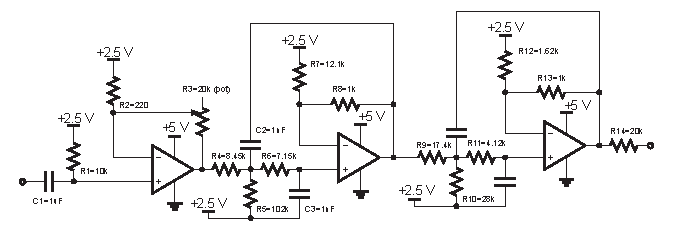
\includegraphics{lpf_sch}
	\caption{Schematic of the active low-pass filter.}
	\label{fig:lpf_sch}
\end{figure}

\begin{figure}
	\centering
	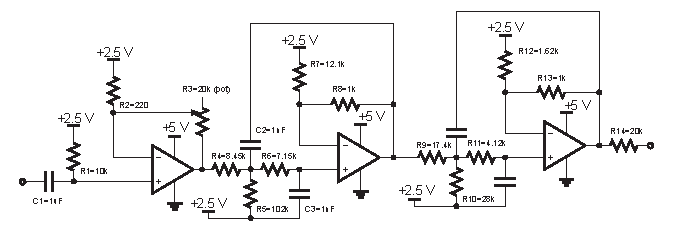
\includegraphics{lpf_sch}
	\caption{Schematic of the active low-pass filter.}
	\label{fig:lpf_pic}
\end{figure}


\subsubsection{Gain stage}

We will use the Texas Instrument OPA4228 quad Op-Amp for both the gain stage and the active LPF. A pinout diagram of OPA4228 is shown in Fig. 6.10.4.

Identify the gain stage of the audio amplifier from Fig. 6.10.1. What is the expression of its gain? Notice the +5V bias does not affect this result, rather it simply shifts the bias of the overall amplifier since a single 9V supply (battery) is used vs a double +/- supply.
Build just the gain stage of the audio amplifier. Remember to power the op-amp chip by using 9V for V+ and ground for V-. Use the 9V battery as the supply for all the measurements to achieve better noise performance. Remember to disconnect the battery when measurements are not being made.
The gain is controlled using a 20 kΩ potentiometer (POT). To test the circuit, input a 1-kHz 100 mVp-p sine wave to the IF input using a signal generator. What is the maximum gain before clipping occurs, and what is the corresponding peak-to-peak voltage at the output?
The audio card on a typical laptop is designed to take in line level signals. Notice that this limits the sound card input signal strength to approximately 3 Vp-p. Adjust the pot to achieve 3 Vp-p on the oscilloscope at 1 kHz. Tabulate and plot the gain from 100 Hz to 3 MHz while keeping the pot fixed. Find the 3-dB cutoff frequency or the 3-dB bandwidth at this gain. Use at least 20 data points.

\subsubsection{Active LPF}
Build the rest of the audio amplifier circuit, i.e. the active LPF. To measure just the filter response, disconnect R4 and R14 from the circuit (Fig. 6.10.1). Input a 3-Vp-p signal in place of R4 and measure the output in place of R14. R14 will only be needed as a current limiting resistor when connecting the amplifier to the laptop’s audio card. Again tabulate and plot the frequency response from 100 Hz to 20 kHz. What is the cutoff frequency of the filter?
The overall filter consists of 2 low pass filters. What is the order of the overall filter and how is it determined from the schematic? Is the bandwidth of the filter tunable? How would one increase or decrease the cutoff frequency?
What limitation does the cut-off frequency of the LPF place on the radar’s performance?  (Hint: what happens when your object is too far away)

\subsubsection{Gain Stage + Filter}
Reconnect R4 (R14 is still disconnected) and measure the overall response of the amplifier. Input a 100 mVp-p sine wave to the IF input. Adjust the pot for a 3 Vp-p output at 1 kHz and once again sweep the frequency from 100 Hz to 20 kHz while tabulating the voltage output and the gain. What is the cutoff frequency? Compare the results to previous measurements. Tabulate and plot all of the results for the report.
Reconnect R14. Break the audio cable and connect the LPF output to the right channel and the SYNC signal (from the modulator) to the left channel. 


\subsection{Analog to digital converter}

\subsection{Signal processing}

Use teensy 3.1 to sample and process data? sounds like too much work...

Using the laptop



\begin{thebibliography}{9}

\bibitem{lamport94}
  Leslie Lamport,
  \emph{\LaTeX: a document preparation system},
  Addison Wesley, Massachusetts,
  2nd edition,
  1994.

\end{thebibliography}

\end{document}